\documentclass{article}
\usepackage{listings}
\usepackage{amsmath}
%\usepackage{subfigure}
\usepackage{subfig}
\usepackage{amsthm}
\usepackage{amsmath}
\usepackage{amssymb}
\usepackage{graphicx}
\usepackage{mdwlist}
\usepackage[colorlinks=true]{hyperref}
\usepackage{geometry}
\usepackage{titlesec}
\geometry{margin=1in}
\geometry{headheight=2in}
\geometry{top=2in}
\usepackage{palatino}
\usepackage{mathrsfs}
\usepackage{fancyhdr}
\usepackage{paralist}
\usepackage{todonotes}
\setlength{\marginparwidth}{2.15cm}
\usepackage{tikz}
\usetikzlibrary{positioning,shapes,backgrounds}
\usepackage{float} % Place figures where you ACTUALLY want it
\usepackage{comment} % a hack to toggle sections
\usepackage{ifthen}
\usepackage{mdframed}
\usepackage{verbatim}
\usepackage[strings]{underscore}
\usepackage{listings}
\usepackage{bbm}
\rhead{}
\lhead{}

\renewcommand{\baselinestretch}{1.15}

% Shortcuts for commonly used operators
\newcommand{\E}{\mathbb{E}}
\newcommand{\Var}{\operatorname{Var}}
\newcommand{\Cov}{\operatorname{Cov}}
\newcommand{\Bias}{\operatorname{Bias}}
\DeclareMathOperator{\argmin}{arg\,min}
\DeclareMathOperator{\argmax}{arg\,max}

% do not number subsection and below
\setcounter{secnumdepth}{1}

% custom format subsection
\titleformat*{\subsection}{\large\bfseries}

% set up the \question shortcut
\newcounter{question}[section]
\newenvironment{question}[1][]
  {\refstepcounter{question}\par\addvspace{1em}\textbf{Question~\Alph{question}\!
    \ifthenelse{\equal{#1}{}}{}{ [#1 points]}: }}
    {\par\vspace{\baselineskip}}

\newcounter{subquestion}[question]
\newenvironment{subquestion}[1][]
  {\refstepcounter{subquestion}\par\medskip\textbf{\roman{subquestion}.\!
    \ifthenelse{\equal{#1}{}}{}{ [#1 points]:}} }
  {\par\addvspace{\baselineskip}}

\titlespacing\section{0pt}{12pt plus 2pt minus 2pt}{0pt plus 2pt minus 2pt}
\titlespacing\subsection{0pt}{12pt plus 4pt minus 2pt}{0pt plus 2pt minus 2pt}
\titlespacing\subsubsection{0pt}{12pt plus 4pt minus 2pt}{0pt plus 2pt minus 2pt}


\newenvironment{hint}[1][]
  {\begin{em}\textbf{Hint: }}{\end{em}}

\ifshowsolutions
  \newenvironment{solution}[1][]
    {\par\medskip \begin{mdframed}\textbf{Solution~\Alph{question}#1:} \begin{em}}
    {\end{em}\medskip\end{mdframed}\medskip}
  \newenvironment{subsolution}[1][]
    {\par\medskip \begin{mdframed}\textbf{Solution~\Alph{question}#1.\roman{subquestion}:} \begin{em}}
    {\end{em}\medskip\end{mdframed}\medskip}
\else
  \excludecomment{solution}
  \excludecomment{subsolution}
\fi

\newcommand{\boldline}[1]{\underline{\textbf{#1}}}

\chead{%
  {\vbox{%
      \vspace{2mm}
      \large
      Machine Learning \& Data Mining \hfill
      Caltech CS/CNS/EE 155 \hfill \\[1pt]
      Miniproject 2\hfill
      Released February $16^{th}$, 2018 \\
    }
  }
}

\begin{document}
\pagestyle{fancy}

\section{Introduction}
\medskip
\begin{itemize}

    \item \boldline{Group members} \\
    Aw Young Qingzhuo, Ola Kalisz, and Riley Patterson

    \item \boldline{Team name} \\
    Not Hotdog

    \item \boldline{Code} \\
    \url{https://github.com/veniversum/cs155-projects}, see especially \texttt{project2/src}

    \item \boldline{Division of labour} \\
    We all independently did the ``basic'' visualizations before deciding on a final view of them to present here.

    Ola implemented the ``off the shelf'' SVD and looked into the difference between using $U,V$ from $Y \sim = U\Sigma V$ vs. $Y \sim = UV$ and into the test error for this vs. the HW5 model.

    Qingzhuo worked with models including biases and created visualizations colored by age and genre.

    Riley worked with models using his hw5 solution and wrote code for finding/labeling outliers in the 2D projections as well as coloring by age, genre, and buckets of genres.

\end{itemize}



\section{Overview}
\medskip
\begin{itemize}

    \item \boldline{Models and techniques tried}

        We visualized a 2D projection of the movies data using each of the following:
        \begin{itemize}
            \item Matrix Factorization as implemented in HW5, where $Y \sim = UV^T$, i.e. $U = U_{SVD}\sqrt{\Sigma}$ and $V = V_{SVD}\sqrt{\Sigma}$.
            \item Matrix Factorization models including bias. % TODO bit more detail here
            \item SVD from SciPy, where we used $U_{SVD},V_{SVD}$ in $Y \sim = U_{SVD} \Sigma V_{SVD}$.
        \end{itemize}

    \item \boldline{Work timeline}
    \begin{itemize}
    \item \textbf{Feb 21:} Riley: code and results from basic visualizations, some helper code for loading features of the movie dataset and querying them
    \item \textbf{Feb 22:} All: worked on various matrix factorization models as described in ``division of work,'' producing many of the plots to be used in the report and exploring lots of possible correlations using interesting colorings and labelings of the graph.
    \item \textbf{Feb 23:} Produced final visualizations and report using learnings from previous day.
        % TODO potentially add more here if we do more
    \end{itemize}

\end{itemize}



\section{Approach}
\medskip
\begin{itemize}

    \item \boldline{Data processing and manipulation}
    % TODO write about how we queried movie features and used them to produce the graphs
    % TODO maybe write about 0- vs. 1-indexing?

    \item \boldline{Details of models and techniques} \\

        % TODO write about hw5 model

        % TODO write about models including bias

        % TODO write about scipy SVD and $V$ vs. $\sqrt{\Sigma}V$

\end{itemize}

\section{Visualizations and Results}
\medskip
\subsection{Basic Visualizations}
\begin{itemize}
    \item \boldline{Histogram of All Ratings in the MovieLens Dataset}

        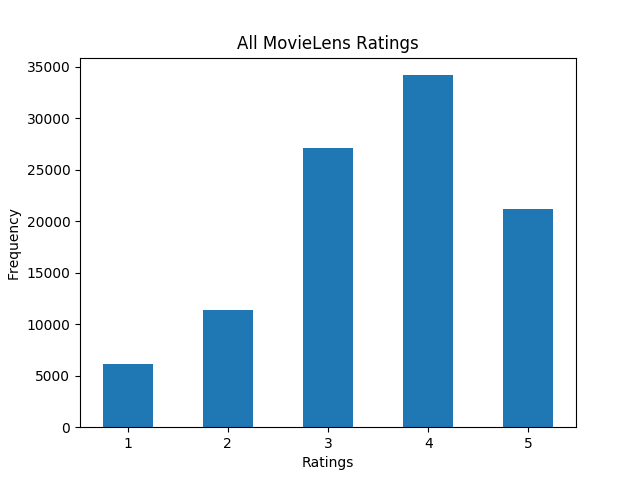
\includegraphics{basics_all.png}

        Here we see a distribution biased towards higher ratings, which suggests either that people have a systematic bias to think all movies are above average or that there's a selection bias in the movies that they end up seeing and rating.

    \item \boldline{Histogram of Ratings for top 10 most frequently rated movies in the MovieLens Dataset}

        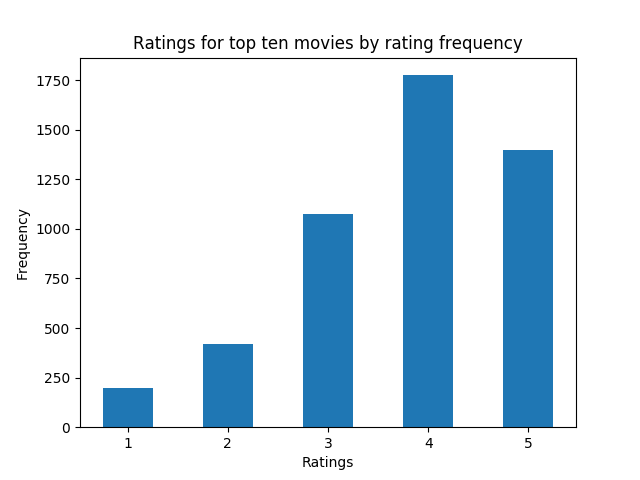
\includegraphics{basics_top_ten_frequency.png}

        Here we see a distribution even more biased towards higher ratings than for all movies, which suggests some form of positive feedback where a movie which receives higher ratings on average also ends up getting more viewers/raters to rate it.

    \item \boldline{Histogram of Ratings for top 10 movies by average rating in the MovieLens Dataset}

        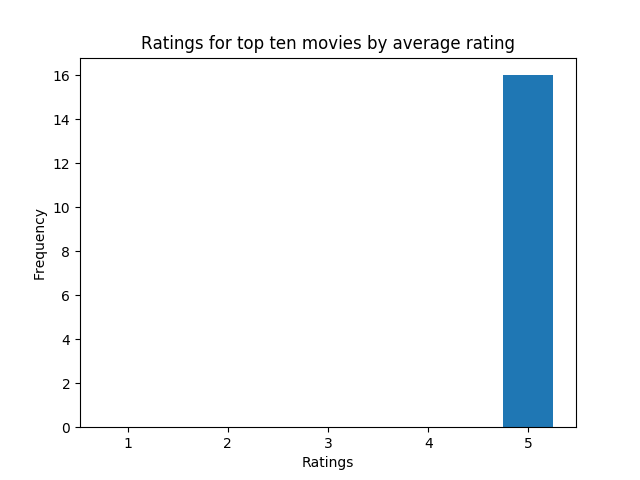
\includegraphics[scale=.5]{basics_top_ten_rated.png}
        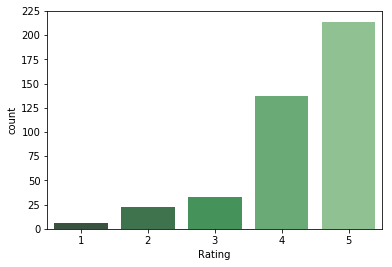
\includegraphics[scale=.5]{basics_top_ten_over50ratings.png}

        When we look at movies that strictly match the definition of highest average rating, we find movies that have been exclusively rated 5 stars, but with very small numbers of ratings each (sometimes just one). We also looked at the top ten movies \textit{having at least 50 ratings}, for which we found a bit more interesting results but still with an obvious strong bias towards higher ratings compared to the whole dataset.

    \item \boldline{Histograms of Ratings for all movies in three different genres}

        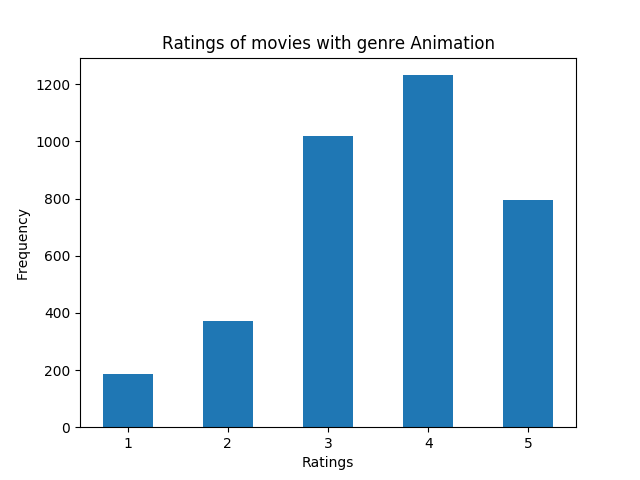
\includegraphics[scale=.25]{basics_genre_Animation.png}
        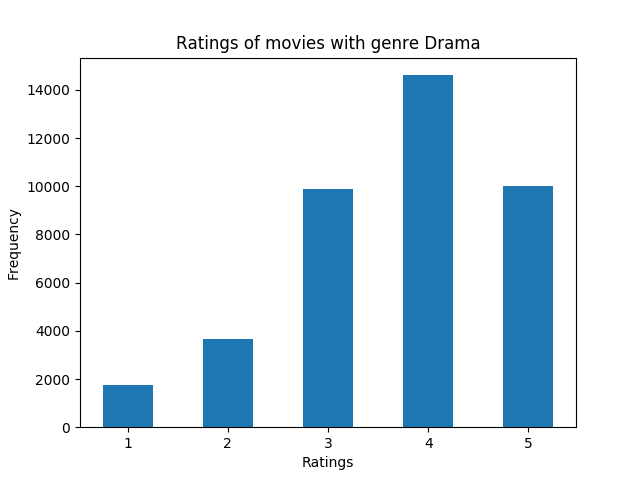
\includegraphics[scale=.25]{basics_genre_Drama.png}
        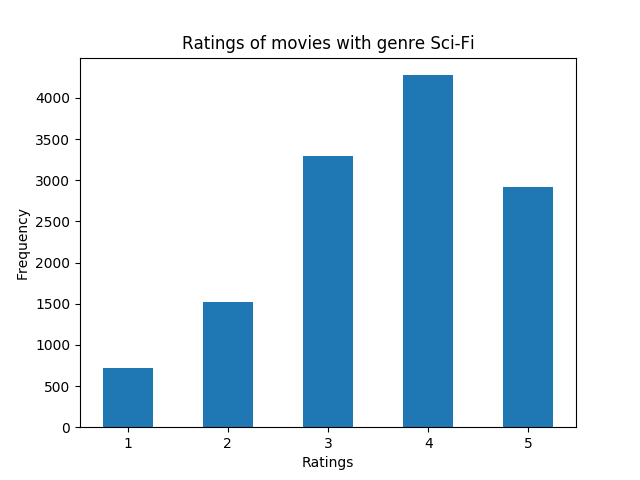
\includegraphics[scale=.25]{basics_genre_Sci-Fi.png}

        Looking at movies from three different genres, we see that Drama movies have the highest proportion of positive (4- and 5-star) reviews among the three, and Sci-Fi movies, while having a larger proportion of 5-star reviews than Animation movies, also have notably greater proportions of 1- and 2-star reviews, exhibiting higher variance of quality and/or taste.

\end{itemize}

\subsection{Matrix Factorization}
\subsubsection{Comparison of Models}
\begin{itemize}
    \item \boldline{HW5 Implementation}
        % TODO parameter details and justification
        % TODO test error and discussion
    \item \boldline{SVD with Bias}
        % TODO parameter details and justification
        % TODO test error and discussion
    \item \boldline{SVD from SciPy with no Bias}
        % TODO parameter details and justification
        % TODO test error and discussion
\end{itemize}

\subsubsection{Visualizations}
\begin{itemize}
    \item \boldline{Ten movies chosen by distance from centroid of scatterplot}

        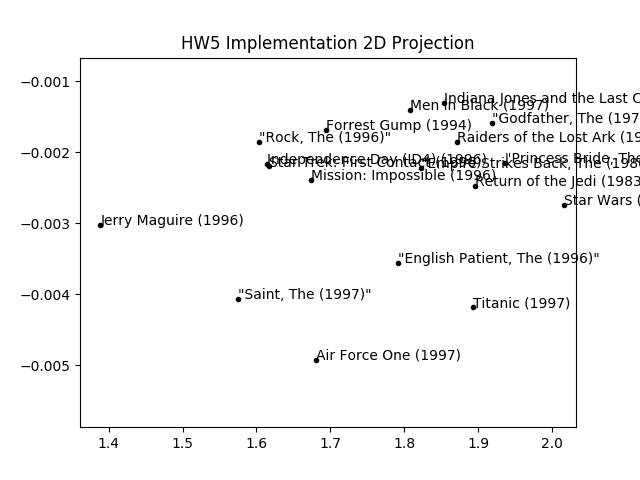
\includegraphics[scale=.5]{hw5_impl_action_romance.png}

        Action and Romance films projected using $V$ from the HW5 implementation of matrix factorization. Here we can see many of the Romance movies in the bottom half of the plot (with the exception of Air Force One), and a cluster of Action movies at the top, suggesting the difference between these genres is correlated with the dimension represented in the y-axis.

        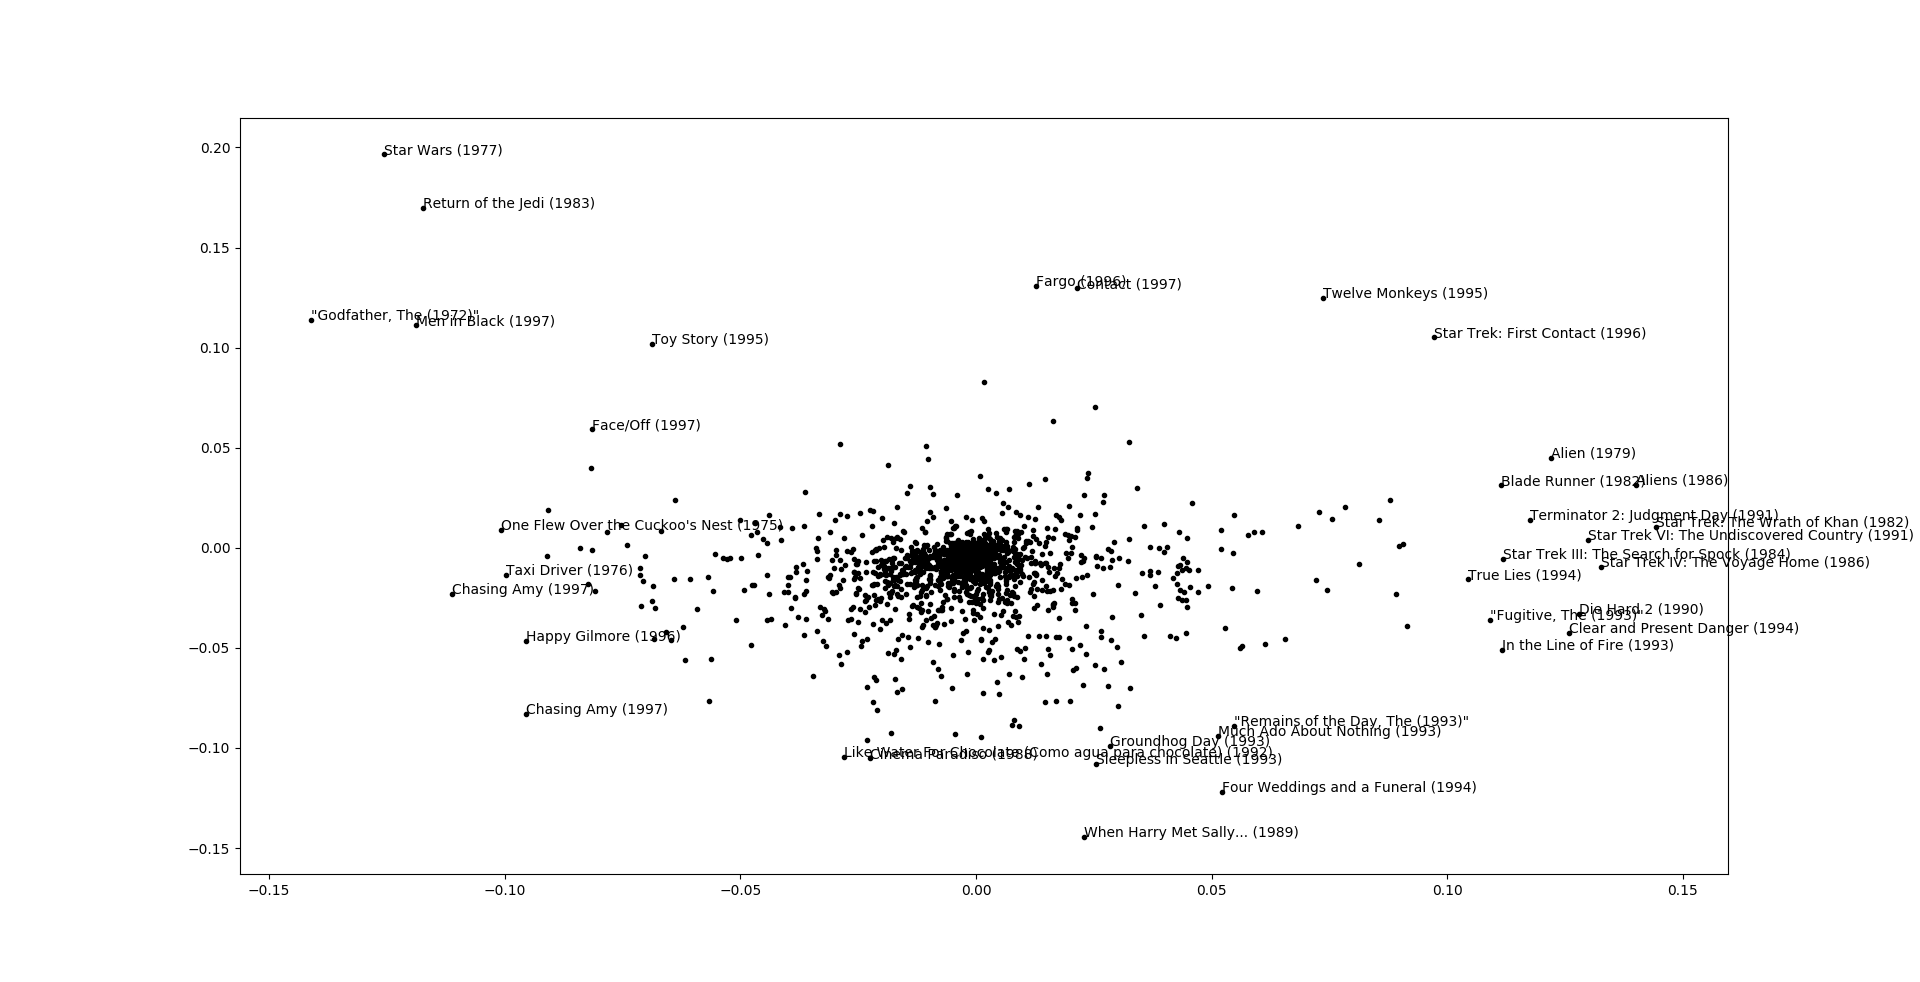
\includegraphics[width=\textwidth]{off_the_shelf_outliers.png}

        All movies projected using $V$ from SciPy SVD, with the most distance movies from the origin labeled. Here we see a number of clusters of similar movies, including comedies in the bottom left, Sci-Fi in the right, and more ``artsy'' movies in the bottom.

        % TODO viz from SVD w/ Bias and commentary
    \item \boldline{Top ten most frequently rated movies}
        % TODO viz from HW5 impl and commentary
        % TODO viz from SVD w/ Bias and commentary

        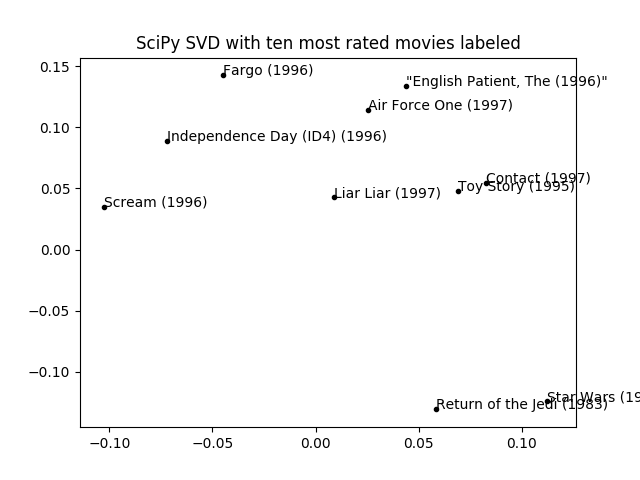
\includegraphics[scale=.5]{scipy_top_ten_frequent.png}

        Top ten most frequently rated movies plotted with the SciPy SVD projection. Here we see a clear cluster in the bottom left where the Star Wars movies appear together, and some distance from the romance movies on top.
    \item \boldline{Highest average rated movies}
        % TODO viz from HW5 impl and commentary
        % TODO viz from SVD w/ Bias and commentary

        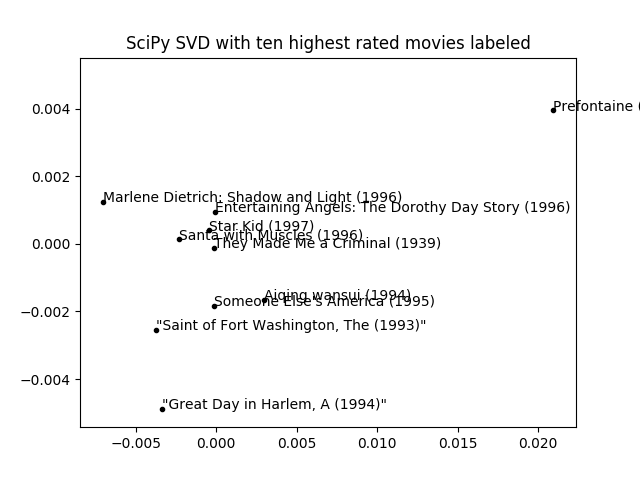
\includegraphics[scale=.5]{scipy_top_ten_rated.png}

        Top ten rated movies plotted with the SciPy SVD projection. Here it is difficult to find a correlation, likely due to the small number of ratings (as few as one) for these movies results in less data to distinguish them.
    \item \boldline{Ten movies from three different genres}
        % TODO viz from HW5 impl and commentary
        % TODO viz from SVD w/ Bias and commentary

        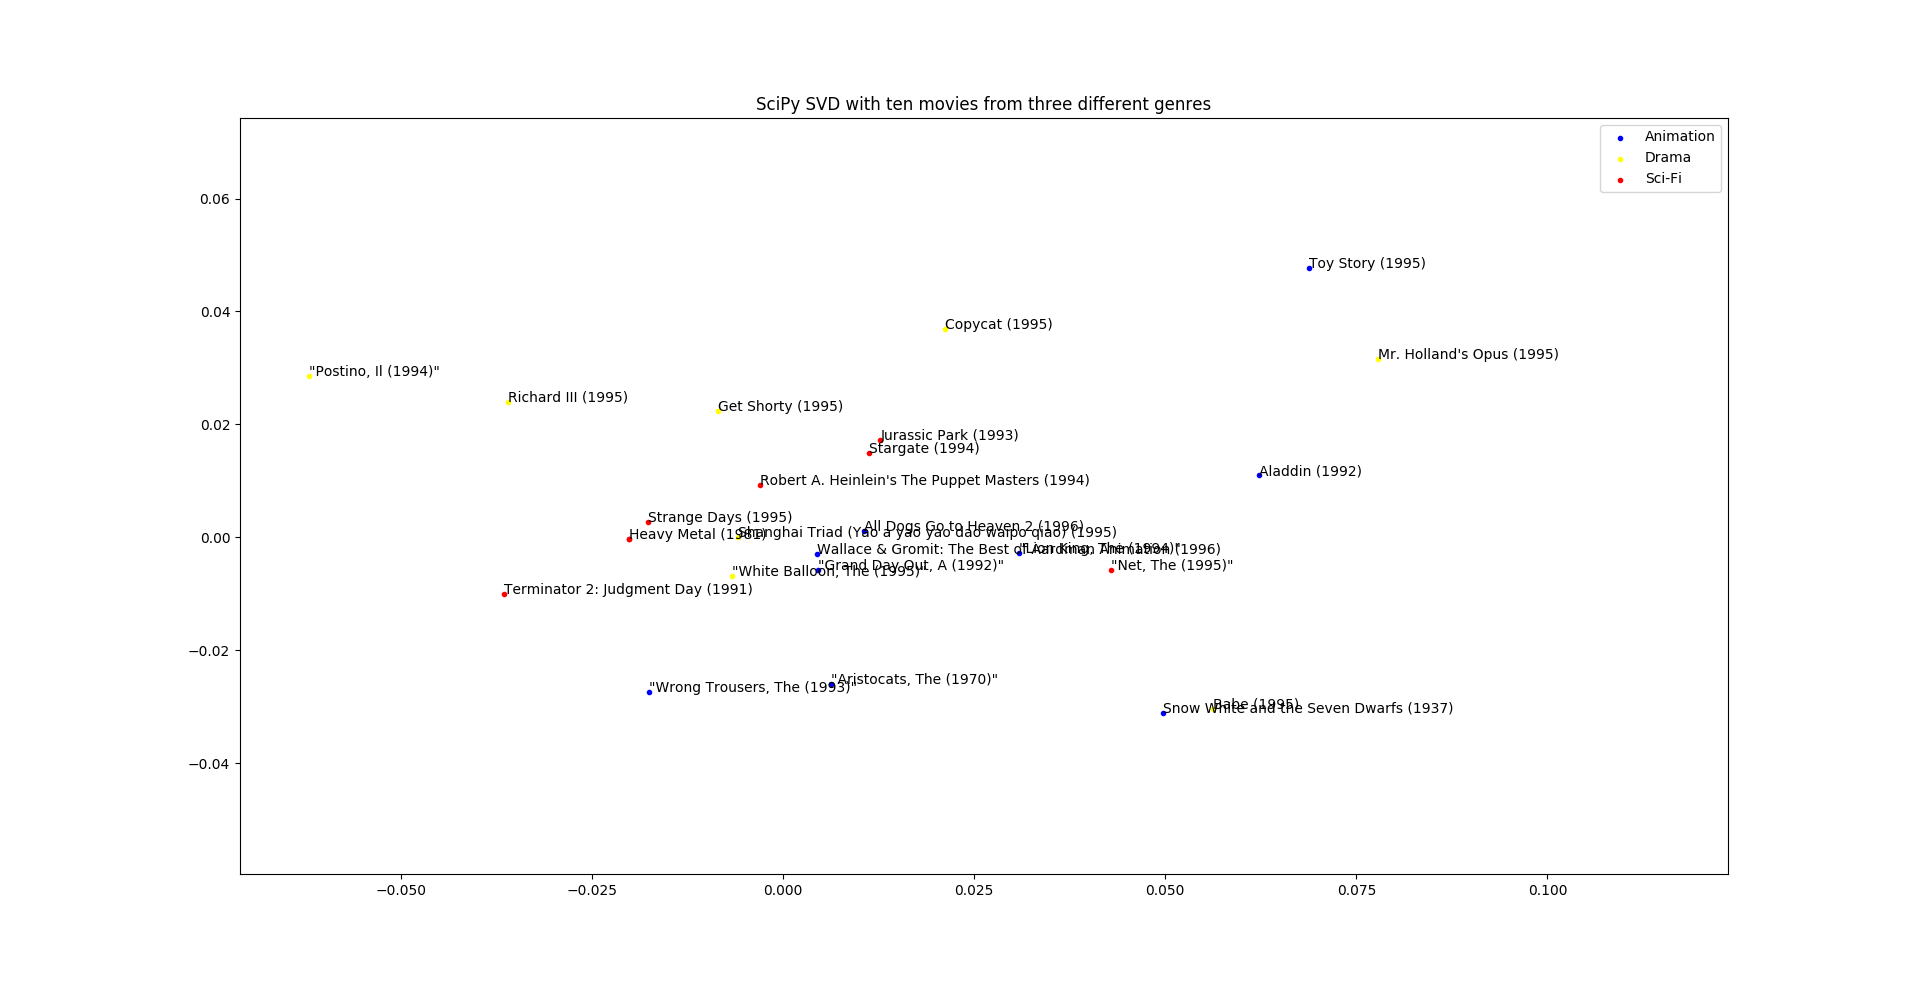
\includegraphics[width=\textwidth]{svd_three_genres.png}

        Ten movies each from Animation, Drama, and Sci-Fi, plotted with the SciPy SVD projection. Here we see that most of the dramas are higher on the y-axis, while Sci-Fi is largely lower on the x-axis  than Animation.
    \item \boldline{Other}

        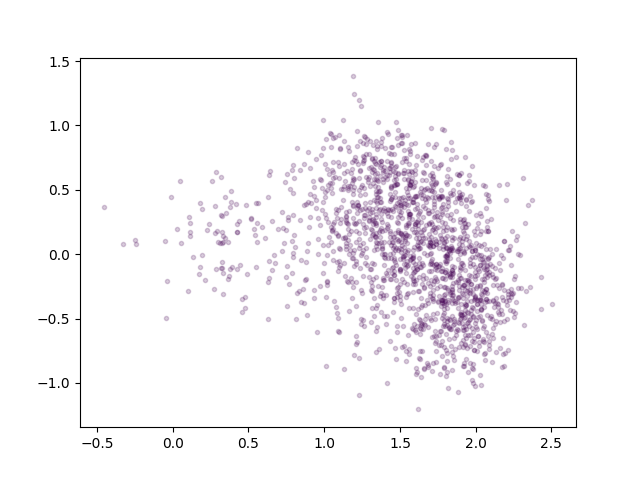
\includegraphics[scale=.5]{age_coloring.png}

        All movies from the HW5 implementation-based 2D projection, colored with more recent movies being darker. Here we see a correlation with age on the x-axis.
\end{itemize}

\section{Conclusion}
\medskip
\begin{itemize}

    \item \boldline{Discoveries} \\
        % TODO

    \item \boldline{Challenges} \\
        % TODO

    \item \boldline{Concluding Remarks} \\
        % TODO

\end{itemize}

\end{document}
